\documentclass[11pt,aspectratio=149]{ctexbeamer}
% 自訂字體的封包
\usepackage{fontspec} 
\setmonofont{CodeNewRomanNerdFontMono-Regular.otf}[Scale=MatchLowercase]
\usepackage{color} 
\usepackage{xcolor}



% 數學工具及符號
\usepackage{mathtools, amsmath, amsfonts, amsthm, latexsym} 

% 定义一个新的计数器
% 导入必要的包
\usepackage{xcolor}
\usepackage[most]{tcolorbox} % 用于创建带有阴影效果的框
\definecolor{myblockbgcolor}{RGB}{241, 241, 255}
\definecolor{Myblue}{RGB}{241, 241, 255}
\definecolor{Default_Blue}{RGB}{52,51,171}
\setbeamercolor{structure}{fg=Myblue} 
% 定义一个新的计数器
\newcounter{defname}

% 自定义问题环境
\newenvironment{mydef}{
  \stepcounter{defname}
  \begin{tcolorbox}[colframe=black, colback=blue!10, title=\textbf{定义 \arabic{defname}}]
}{
  \end{tcolorbox}
}

% 公式
% 自定义tcolorbox代码框样式
% 自定义tcolorbox代码框样式
\newtcolorbox[auto counter, number within=section]{listing}[2][]{%
  colback=yellow!10!white,      % 代码背景色
  colframe=black,                % 代码框框架颜色为黑色
  title=\textbf{代码},           % 标题为加粗的"代码"
  fonttitle=\bfseries           % 标题加粗
}


\usepackage{xcolor} % 如果你需要自定义颜色

% 分別將數學符號間的間隔加大及加粗
\usepackage{newtxtext,newtxmath}

% 圖表自動編號的封包
\usepackage{caption} 

%% 設定自動編號
\setbeamertemplate{caption}[numbered]

% 導入圖形與表格的封包
\usepackage{graphicx}  % \scalebox{} 可用於將過大的表格縮小
\usepackage{booktabs}

% 排列多個子圖形的封包
\usepackage{subfigure} 

% 允許表格的一格能多列呈現的封包
\usepackage{multirow} 

% 可指定表格排版的封包
\usepackage{array}

% 翻轉表格的封包
\usepackage{lscape} 

% 序列標號
\usepackage{enumerate} 

% 繪圖封包 (用於添加浮水印)
\usepackage{tikz}
\usepackage{svg}
\usepackage{float}

% 引注參考資料
\usepackage{natbib}

% 註釋掉大部分的封包
\usepackage{comment}

% 浮水印

% 设置背景模板
\usebackgroundtemplate{%
    \tikz[overlay, remember picture] % 使用 TikZ 创建一个覆盖层
        \node[opacity=0.1, anchor=center, at=(current page.center)] % 设置透明度和位置
            {
\includegraphics[scale=0.0618]{Fig/上海财经大学-logo-2048px.png}}; % 载入并缩放图片
}

\mode<presentation>{
%\usetheme{default}
%\usetheme{AnnArbor}
%\usetheme{Antibes}
%\usetheme{Bergen}
%\usetheme{Berkeley}
%\usetheme{Berlin}
% \usetheme{Boadilla}
% \usetheme{CambridgeUS}
% \usetheme{Copenhagen}
%\usetheme{Darmstadt}
%\usetheme{Dresden}
%\usetheme{Frankfurt}
%\usetheme{Goettingen}
%\usetheme{Hannover}
%\usetheme{Ilmenau}
%\usetheme{JuanLesPins}
%\usetheme{Luebeck}
\usetheme{Madrid}
%\usetheme{Malmoe}
%\usetheme{Marburg}
%\usetheme{Montpellier}
%\usetheme{PaloAlto}
%\usetheme{Pittsburgh}
%\usetheme{Rochester}
%\usetheme{Singapore}
%\usetheme{Szeged}
%\usetheme{Warsaw}
\usetheme[style=light]{Nord}

%----------------------------------------------------------------------------------------
%	外框形式 (擇一,不選等同選擇默認的外框形式)
%----------------------------------------------------------------------------------------

\useoutertheme{default}
% \useoutertheme{infolines}
% \useoutertheme{miniframes}
% \useoutertheme{smoothbars}
%\useoutertheme{sidebar}
%\useoutertheme{split}
% \useoutertheme{shadow}
% \useoutertheme{tree}
% \useoutertheme{smoothtree}

%----------------------------------------------------------------------------------------
%	外框的自訂義調整 
%----------------------------------------------------------------------------------------

% 外框上緣的字 (fg) 為黑色,背景 (bg) 為白色。
%\setbeamercolor{section in head/foot}{fg=white, bg=black} 

% 外框上緣顯示的章節(section)頁數標籤是否關閉
% \setbeamertemplate{mini frames}{}   

% 調整外框形式的字體大小
\setbeamerfont{headline}{size=\scriptsize}
\setbeamerfont{footline}{size=\scriptsize}

% 取消右下方的跳轉工具列
%\setbeamertemplate{navigation symbols}{} 

% % 自定義1:外框下緣僅出現名字及頁碼
% \setbeamertemplate{footline}
% {\leavevmode%
% \hbox{%
% \begin{beamercolorbox}[wd=0.5\paperwidth,ht=3ex,dp=1ex,leftskip=2ex]%
% {author in head/foot}%
% {\footnotesize\textbf{\insertshortauthor}}%
% \end{beamercolorbox}%
% \begin{beamercolorbox}[wd=0.5\paperwidth,ht=3ex,dp=1ex,right]%
% {author in head/foot}%
% \footnotesize \textbf{{\insertframenumber{} / \inserttotalframenumber\hspace*{2ex}}} %頁碼控制選項
% \end{beamercolorbox}%
% }}

%% 自定義2:清除外框下緣但僅出頁碼
%\setbeamertemplate{footline}[page number] 

%% 自定義3:清除外框下緣
%\setbeamertemplate{footline}[] 

%----------------------------------------------------------------------------------------
%	顏色主題 (擇一,不選等同選擇默認的顏色主題)
%----------------------------------------------------------------------------------------

% \usecolortheme{default}
%\usecolortheme{albatross}
% \usecolortheme{beaver}
%\usecolortheme{beetle}
%\usecolortheme{crane}
% \usecolortheme{dolphin}
\usecolortheme{dove}
% \usecolortheme{fly}
% \usecolortheme{lily}
%\usecolortheme{orchid}
 % \usecolortheme{rose}
%\usecolortheme{seagull}
%\usecolortheme{seahorse}
% \usecolortheme{whale}
%\usecolortheme{wolverine}
% \usecolortheme{spruce}
%----------------------------------------------------------------------------------------
%	顏色主題的自訂義調整 
%----------------------------------------------------------------------------------------

% 全文的主題色 (可以特別針對報告對象或機構的代表色調整!)
% \setbeamercolor{structure}{fg=Myblue} 

% 封面頁中標題區塊的底色及字體顏色
%\setbeamercolor{title}{bg=green, fg=black} 

% 各頁標題區塊的底色及字體顏色
%\setbeamercolor{frametitle}{bg=white,fg=black} 

% 全文的內文顏色
%\setbeamercolor{normal text}{fg=orange}

% 數學區塊的標題顏色 
%\setbeamercolor{block title}{bg=blue,fg=yellow} 

% 數學區塊的內文顏色 
%\setbeamercolor{block body}{bg=green,fg=red} 

% 警示文字的顏色
\setbeamercolor{alerted text}{fg=red} 

%----------------------------------------------------------------------------------------
%	enumerate 及 item 的形狀
%----------------------------------------------------------------------------------------

%\useinnertheme{rounded} % 圓球 (3D)
\useinnertheme{circles} % 圓形 (2D)
%\useinnertheme{rectangles} % 方形
% \useinnertheme{triangle} % 三角形
%\useinnertheme{inmargin} % 插入邊沿
\setbeamertemplate{itemize items}[triangle]

%----------------------------------------------------------------------------------------
%	自訂 item 的顏色
%----------------------------------------------------------------------------------------

%\setbeamercolor{item projected}{bg=red}

%----------------------------------------------------------------------------------------
%	個人化的設置及細節調整
%----------------------------------------------------------------------------------------

% 設定頁面邊界
\setbeamersize{text margin left=  0.75cm, text margin right= 0.75cm}
\special{papersize=\the\paperwidth,\the\paperheight}
\providecommand{\tabularnewline}{\\}
}


\linespread{1.5}
\newcommand{\textred}[1]{\textcolor{red}{#1}}
\title{社区识别}
\subtitle{基于无桩共享单车“潮汐”特征的时空聚类}
\author{张浩怡、潘凌志}
\date{\today}
\usepackage{graphicx}

\begin{document}

% 封面页
\begin{frame}[plain,noframenumbering]
    \maketitle
\end{frame}

% 目录页

\begin{frame}[plain]
\tableofcontents
\end{frame}

\section{引言}

% 1. 研究背景:为什么要研究这个
% 2. 历史背景:这方面,之前的人都是怎么做的
% 3. 研究问题:我们的研究问题是什么
% 4. 研究亮点:展示我们的研究方法、研究结果中的亮点部分

\begin{frame}{研究背景}
上海市的共享单车企业主要采用\textred{无桩共享单车}的运营模式,这在为市民生活提供便利的同时,也因单车在地区间的流入流出具有较大的随机性和不确定性,导致了显著的\textred{“潮汐”现象}。考虑以下情形:
\begin{enumerate}
\item 期末周的晚上 10 点,你从图书馆出来,想骑单车回宿舍,一眼望去\textred{找不到一辆}……
\item 周末外出游玩,偶遇早晚高峰,地铁站附近\textred{停满了单车},拼尽全力无法战胜,只好把车停得远远的……
\end{enumerate}

如何通过数据挖掘和商务分析来\textred{识别}城市中不同区域和时段的需求模式和规律?进而为公司的\textred{短期运营和长期决策}提供建议?
\end{frame}

\begin{frame}{相关工作}
相较于无桩共享单车,有桩共享单车的出现时间较早,且固定停车桩位一定程度上化简了问题,因此对有桩情形的研究也是相对详细的。
\begin{columns}[T]
\begin{column}{0.48\textwidth}
\begin{itemize}
    \item \textit{一类注重于影响公共自行车用车量的时间因素。如El-Assi等(2017)基于经验探讨了有桩共享单车系统的使用模式,包括早晚高峰期间的租还车行为。}
\end{itemize}

\end{column}
\begin{column}{0.48\textwidth} 
\begin{itemize}
    \item \textit{一类探索如何通过数据分析来识别热点区域。罗桑扎西(2018)等通过构建缓冲区并采用多元回归的方法,探究了南京市共享单车的影响因子。}
\end{itemize}
\end{column}
\end{columns}
 \vspace{0.5cm} % 在 columns 环境之后增加垂直间距
随着数据收集技术的发展,研究开始利用大数据分析来识别热点区域。
\end{frame}

\begin{frame}{技术路线}
\begin{quote}
把房子点燃,将未知的问题转化为已知的问题
\end{quote}


\begin{mydef}
\begin{enumerate}
    \item \textit{将复杂的个体出行网络信息转换到易于分析的地理栅格上}。
    \item \textit{对于包含时空信息的地理栅格,以图的视角,构建相关性网络}。
    \item \textit{类比网络图结构中的社区探测问题,实现聚类,发现社区组群}。
    \item \textit{寻找社区中心,作为共享单车区域规律的中心代表}。
\end{enumerate}
\end{mydef}
\end{frame}

\begin{frame}{研究亮点}
\begin{itemize}
    \item 在数据预处理方面,时间要素了构建\textred{时间}、\textred{距离}、和\textred{速度}三特征,根据商业公司的\textred{实际运营策略}进行数据清洗;空间要素则使用\textred{核密度分析方法}构建了 \textred{POI 指数}来表征各个停车点的社会地理环境。
    \item 在数据建模分析方面,整合多方数据,既考虑了时间要素,又综合地理要素,构建了\textred{更加丰富的特征信息}用以聚类,更贴近实际情况。
    \item 在完成社区划分的基础上,进一步挖掘了社区的潮汐特征,成功识别并定位了单车使用的\textred{热点区域},提供了观察城市发展的\textred{新视角}。
    \item 整体实验呈现明显的模块化,具有很好的\textred{移植性},进而研究其他城市的若干特征。
\end{itemize}




\end{frame}

%以前都是直接用\includegraphics[]{}的,好的新奇的用法(
% bur 哥们,现在写的才对,外面套了个figure
% 实在不想截图吧
% 没有改变
%似乎几个方法调不了大小是为什么,你那边编译后大小有改变吗?
%怪的
%那个表格是不是需要截屏?
%  其实不用照搬原论文,按自己汇报的习惯来写最后
%数据包含 2021 年 1 月 至 8 月 的部分共享单车订单数据,共 8 个数据项,数据类型均为字符串型//这个地方要不要改成2019-2021年?
% 艹我还以为你和我说话
% 难绷 /≡[。。]≡
%我是在想原论文需不需要改,你就说数据来源就行,剩下的在时间特征那边再说你做了抽样
% 改了数据抽样不就白写了 我不允许╰(‵□′)╯
%还好吧加一句选取2021年?好像其他是一样的,因为担心会不会有错误,数据大小或者前后矛盾一类的?
%星

\section{数据预处理与EDA}

% 1. 数据来源:简单介绍数据来源和字段含义以及用处
% 2. 时间特征挖掘:介绍运行距离、运行时间、运行速度的构造,实现数据清理
% 3. 地理特征挖掘:POI与 POI 指数
% 注意图片的展示!

\begin{frame}{数据来源}
本项目所用到的数据主要来自两部分:
\begin{enumerate}
\item 深圳市政府数据开放平台(下称平台,相关链接: \href{https://opendata.sz.gov.cn/data/api/toApiDetails/29200_00403627}{https://opendata.sz.gov.cn})。数据集包含2021 年 1 月 至 8 月 的共享单车订单,包括8个字符串型的数据项。
\item 深圳市土地使用情况兴趣点(POI,Point of Interact)。来源于公开网络平台 POI 数据(相关链接:\href{https://www.poi86.com/poi/amap/city/440300.html}{https://www.poi86.com})。数据包含 2021 年深圳市各区的土地使用情况。共 23 种使用用途,包括森林用地,居民小区用地等。
\end{enumerate}
\end{frame}

数据集构成如下表所示,
% 插入图片begin{figure}
\begin{figure}
    \centering
    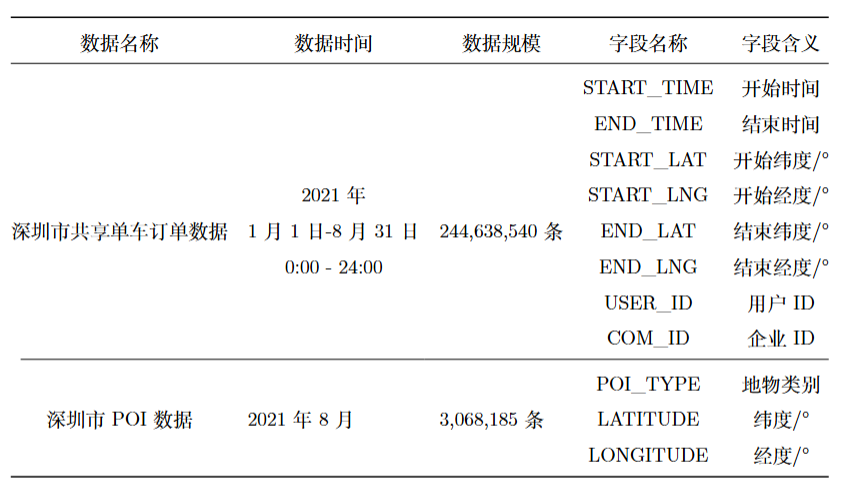
\includegraphics[width=0.8\linewidth]{Figs/数据格式.png}
    \label{fig:enter-label}
\end{figure}

\begin{frame}{时间特征挖掘}
    \begin{itemize}
        \item 数据抽样:首先我们根据天气等因素,对大量的订单数据进行了抽样,选取了8 月中旬(11 日至 18 日)作为实验数据。
        \item 数据清理:
        \begin{enumerate}
            \item 运行距离:
            \item 运行时间:
            \item 运行速度:
        \end{enumerate}
    \end{itemize}
\end{frame}

\begin{frame}{地理特征挖掘}
    
\end{frame}

\section{数据建模分析}
% 1. 已有方法的缺陷
% 2. 相关性网络的构建
% 3. 基于时空约束的网格聚类
% 4. 社区中心的选择(尚未完成)

\section{实验与结果分析}
% 1. 全市尺度效果
% 2. 栅格尺度效果
% 3. 社区尺度效果

\section{实践价值与展望}

% 1. 总结实践方法
% 2. 实践的优点
% 2. 实践的不足

\begin{frame}{实践价值}

\begin{enumerate}
    \item 在数据预处理方面,通过整合POI数据和订单数据,将不易处理的时间序列数据转化为直观易处理的面板数据,实现了地理栅格化;
    \item 在实现栅格化的基础上,进一步实现了相关性网络的构建,将栅格之间的位置、社会环境以及历史订单相似信息归一到边权矩阵中,具有可迁移性;
    \item 之后,类比网络图结构中的社区探测问题,实现了高效的网格聚类,有效探索出不同区域的单车使用情况与流动规律,
    \item 针对热点区域进行单车潮汐特征挖掘,侧面反映了城市发展潜力,为共享单车短期运营和长期决策提供科学支持。
\end{enumerate}

\end{frame}

\begin{frame}{不足与展望}
\begin{enumerate}
    \item 我们在初步处理大规模数据集便面临了性能瓶颈。未来可以引入更高效的图计算框架(如图神经网络)以及并行计算方法,进一步提升算法的计算效率。

    \item 在运行代码中,有大量的重复性繁琐操作,可以进一步探讨方法的泛化能力和跨城市迁移能力,以提升其在不同场景下的适用性。
    
    \item 本文主要基于时空数据和土地使用类型,未来可以进一步引入更多维度的影响因素,如天气变化、道路条件、居民收入水平等,构建更全面的共享单车使用模型。

    \item  未来可以进一步研究其与公交、地铁等其他交通方式的协同效应,探索如何通过多模式交通的联动优化,实现城市资源的最优配置。
\end{enumerate}
\end{frame}

\begin{frame}[plain]

{\Huge THANK YOU !!!}


\vspace{2cm}
我们的项目代码已在 \texttt{github} 上开源,仍在不断完善,地址为 \href{https://github.com/HaoiJhang/Shared-Bike-Mining.git}{\texttt{https://github.com/HaoiJhang/Shared-Bike-Mining.git}}
\end{frame}
\end{document}
